\chapter{Methodology}

\label{chapter4}

In this chapter, we discuss about the techniques and methods used to devise an experiment involving a Pt-Cu bilayer system and subsequently investigate the effect of spin current via SHE.

\section{Experimental plan} \label{sec:plan}

In earlier studies, it has been shown that a pure spin current can be generated and manipulated via a heavy metal through SHE \cite{hirsch1999spin,sinova2004universal,zhang2000spin}. The detection of this spin current can only be done via conversion into charge current (which is measurable) using ISHE. This generally involves a ferromagnetic layer or a magneto-optical method \cite{kimura2007room,li2019spin,stamm2017magneto}.

In our study, we intend to explore the detection of spin current in a NM/HM bilayer system without a magnetic layer, i.e. via electrical means such as using a simple voltmeter.

In many studies involving the electrical detection of spin current, pure spin current is generated using a ferromagnet, which then gets converted to charge current via ISHE, and is hence, detectable using a voltmeter.

Contrary to the above method, we do not generate pure spin current beforehand, but rather provide a pure charge current as supply to our sample, which is converted to spin current via SHE and is converted back to charge current via ISHE. Keeping this in mind, we design our sample accordingly.

\section{Preparation of sample}

We prepare a trilayer system, using copper (Cu) as the NM and platinum (Pt) as the HM. Here, we sandwich a layer of Cu between two layers of Pt. This is depicted in \cref{layers}.

\begin{figure}
    \centering
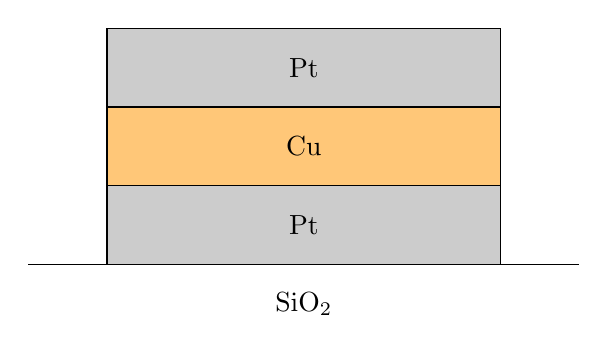
\begin{tikzpicture}
    \draw [fill={rgb:black,1;white,4}] (0,0) rectangle (5,3);
    \node at (2.5,2.5) {Pt};
    \draw [fill={rgb:orange,1;yellow,2;pink,5}] (0,0) rectangle (5,2);
    \node at (2.5,1.5) {Cu};
    \draw [fill={rgb:black,1;white,4}] (0,0) rectangle (5,1);
    \node at (2.5,0.5) {Pt};
    \draw (-1,0) -- (6,0);
    \node at (2.5,-0.5) {SiO$_2$};
\end{tikzpicture}
    \caption{Side view of the trilayer sample}
    \label{layers}
\end{figure}

Now, as mentioned in \cref{sec:plan}, we intend to make the shape of our sample to facilitate the conversion to charge to spin current and vice versa.
Now, as seen in %insert section depicting SHE and ISHE regarding perpendicular conversion
we see that converted spin current, flows perpendicular to the original charge current and similarly during the back conversion via ISHE.
For this, an obvious structural shape would be a path that has two paths, connected via a link being perpendicular to both the paths simultaneously.
Hence, a "H"-like structure comes to mind, which is implemented in our experimental setup.

\subsection{Photolithography}

\begin{figure}[h!]
    \includegraphics[width=\columnwidth]{newtrack.png}
    \caption{Patterned Cu/Pt sample}
\end{figure}

\subsection{Magnetron sputtering}

Through this method, the layer of Cu and Pt are deposited on the Si$O_2$ wafer at an even thickness, to make the whole sample.


% TODO: Finish sample preparation section

\section{Measurement}

After the sample is prepared, we pass electrical (pure charge) current through one arm of the \textit{H}-structure and make voltage measurements across the opposite ends of the sample, as shown in \cref{fig:measurement} . This is commonly called a non-local measurement.

\begin{figure}
\centering
    \begin{circuitikz}[american]
    \draw[thick] (0,0) rectangle (4,10);
    \draw[thick] (0,4.5) -- (-3,4.5);
    \draw[thick] (4,4.5) -- (7,4.5);
    \draw[thick] (0,6) -- (-3,6);
    \draw[thick] (4,6) -- (7,6);
    \draw[thick] (-3,4.5) -- (-3,6);
    \draw[thick] (7,6) -- (7,4.5);
    \draw (-3,5.25) -- (-4,5.25);
    \draw (-4,-1)
    to[isource, l=$I$] (-4,5.25);
    \draw (-4,-1) -- (2,-1);
    \draw (2,-1) -- (2,0);
    \draw (2,10) -- (2,11);
    % \draw (2,11) -- (8,11);
    \draw (2,11)
    to[V, l=$V$] (8,11);
    \draw (8,11) -- (8,5.25);
    \draw (8,5.25) -- (7,5.25);
\end{circuitikz}
    \caption{Pure charge current is supplied across the left arm and the potential difference is measured across the right arm of the sample.}
    \label{fig:measurement}
\end{figure}
